\documentclass[9pt]{extarticle}
\usepackage[utf8]{inputenc}
\usepackage[T1]{fontenc}
\usepackage[letterpaper, portrait, margin=1in]{geometry}
\usepackage{pdflscape}

\usepackage{tgpagella}
\fontfamily{qpl}

\usepackage{siunitx, amsmath, amssymb, hyperref} 
\usepackage{graphicx, float, subcaption, adjustbox}

\setlength{\parindent}{0pt}
\setlength{\parskip}{0.5em}
\setlength{\tabcolsep}{0.5em}
\renewcommand{\arraystretch}{1.5}

% Symbols
\newcommand{\N}{\mathbb{N}}
\newcommand{\R}{\mathbb{R}}
\newcommand{\F}{\mathcal{F}}
\newcommand{\C}{\mathbb{C}}
\newcommand{\D}{\mathcal{D}}
\newcommand{\La}{\mathcal{L}}

% Operators
\DeclareMathOperator{\cis}{cis}
\DeclareMathOperator{\dd}{d}

\newcommand{\inner}{\cdot}

% look nicer than default commands with scaled brackets
\renewcommand{\angle}[1]{\langle#1\rangle}
\newcommand{\Angle}[1]{\left<#1\right>}
\newcommand{\bra}[1]{\langle#1}
\newcommand{\ket}[1]{|#1\rangle}
\newcommand{\Si}[1]{\,\si{#1}}

\renewcommand{\vec}[1]{\mathbf{#1}}
\newcommand{\dv}[3][]{\frac{\dd ^{#1} #2}{\dd #3 ^{#1}}}
\newcommand{\dt}[2][]{\dv[#1]{}{#2}}
\newcommand{\pdv}[3][]{\frac{\partial ^{#1} #2}{\partial #3 ^{#1}}}
\newcommand{\pdt}[2][]{\pdv[#1]{}{#2}}
\newcommand{\pddv}[3]{\frac{\partial^{} #1}{\partial #2 \partial #3}}

\usepackage{multicol}
\usepackage{xifthen}
\usepackage[shortlabels, inline]{enumitem}
\usepackage{biblatex}
\usepackage{siunitx}

\addbibresource{sources.bib}

\renewcommand{\vec}[2][]{\ifthenelse{\isempty{#1}}{\boldsymbol{#2}}{\boldsymbol{#2}^{(#1)}} }


\begin{document}
\begin{center}
	\LARGE \bf Three-Dimensional Vehicle Model
\end{center}
Vehicle Dynamics Final Project \hfill Yevgeniy Gorbachev (2245 Spring)

\begin{multicols*}{2}
\section{Model overview}
The vehicle model aims to reproduce traction-limited acceleration, load
	transfer, and body roll in driving, cornering, and braking. It represents
	the car as a 6-DOF inertia with constant mass \(m\) and body-fixed inertia
	tensor \([\vec[b]{I}]\). Each contact point's vertical force is developed by
	a linear spring (\(k\)) and damper (\(c\)) that are switched off if the
	spring is in `tension'. The wheel has a rotational inertia
	\(J\) and spin \(\omega\) (though no mass) and exerts traction using the
	slip parameter. Finally, cornering force comes from the side-slip angle.
	In total, there are ten degrees of freedom: six from the car body and one
	for the spin of each wheel.

\begin{figure}[H]
	\centering
	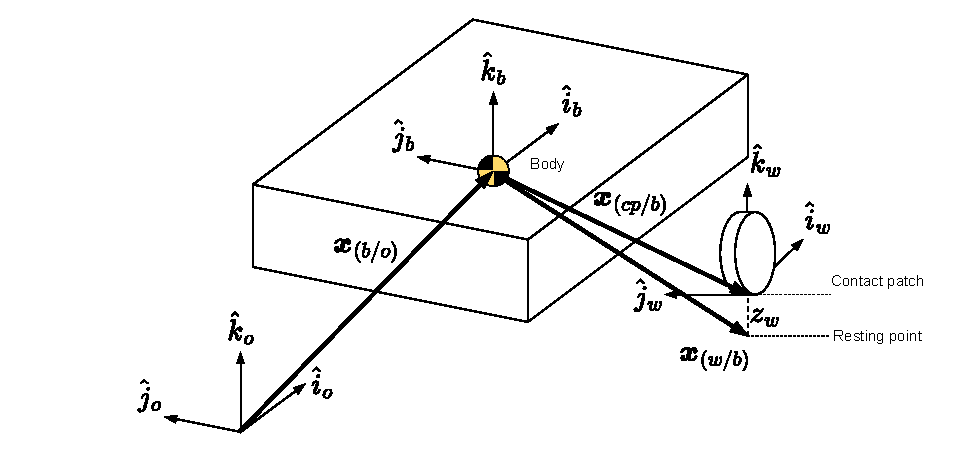
\includegraphics[width=\linewidth]{fig/frames.pdf}
	\caption{Frame definitions}
	% \label{fig:frames}
\end{figure}

The model defines six frames; the inertial `\(o\)', body-fixed `\(b\)', and one
for each wheel. A quantity expressed in a specific coordinate system takes the
	superscript (for example) \([\vec[b]{I}]\).

\subsection{6-DOF Kinetics}

All forces are ultimately calculated in the global (`\(o\)') frame and applied
	using linear momentum balance. Two time integrals of \(\vec{a}_b\) give
	position.

\begin{equation} \label{eq:lmb}
	\sum \vec{F} = m \vec{a}_{b}
\end{equation}

Angular kinetics is less straightforward. Starting with angular momentum balance
about the center of gravity (\(b\)) \cite{hibb},

\begin{equation}\label{eq:amb}
	\sum \vec{M}_{b} = \dot{\vec{H}}_{b} 
		= [\vec{I}_b] \vec{\alpha}_b + 
		\vec{\omega}_b\times([\vec{I}_b]\vec{\omega}_b)
\end{equation}

The model represents orientation with a quaternion which rotates a vector in
	body-fixed axes to inertial axes

\begin{equation}\label{eq:quatconvention}
	\vec[o]{x} = \vec{q}_b \vec[b]{x}
	\vec{q}_b^{-1}
\end{equation}

The car's rotational inertia is a constant in body-fixed
	axes, but all equations of motion are executed in inertial axes. The
	transformation matrix \(R(\vec{q})\) implements the quaternion rotation
	\(\vec{q}_b \vec{v} \vec{q}^{-1}\), which is applied to the body-fixed
	inertia tensor:

\begin{equation} \label{eq:inertia}
	[\vec[o]{I}] = R(\vec{q}_b)^{-1} [\vec[b]{I}] R(\vec{q}_b)
\end{equation}

Then we can re-arrange Eq. \ref{eq:amb}:
\begin{equation} \label{eq:alpha}
	\vec[o]{\alpha}_b = [\vec[o]{I}]^{-1} 
	\left(\sum \vec[o]{M}_b - \vec[o]{\omega}_b \times([\vec[o]{I}_b]\vec[o]{\omega}_b \right)
\end{equation}

\(\vec[o]{\alpha}\) integrates once to \(\vec[o]{\omega}\). The derivative
of orientation is calcualted from angular velocity by \cite{quats}:

\begin{equation} \label{eq:dquat}
	\dot{\vec{q}_b} = \frac{1}{2} \vec[o]{\omega}_b \vec{q}_b
\end{equation}

The bulk of the complexity is combining quantities in different frames
appropriate to each force model.

\subsection{Load}
Each contact patch is described by a constant resting position
\(\vec[b]{x}_{(w/b)}\). If the ground is described by \(z\equiv 0\), the
location of the resting position in inertial axes is 
\begin{equation}
	\vec[o]{x}_{w/o} = \vec[o]{x}_{b/o} + 
	\vec{q}_b \vec[b]{x}_{(w/b)} \vec{q}_b^{-1}
\end{equation}

The elevation of the resting point \(z_w \triangleq \vec[o]{x}_{w/o} \cdot
\hat{k}_o\) gives the compression of the suspension. To find the damping, we
need the vertical velocity of the contact patch. We calculate the displacement
of the contact patch relative to the CG by moving the resting offset straight up
to ground level as \(\vec[o]{x}_{cp/b}=\vec[o]{x}_{w/b} - z_w\hat{k}_o\). This
is inaccurate in a high body roll condition. Then the translational velocity of
the contact patch is given by:

\begin{equation}
	\vec[o]{v}_{w/o} = \vec[o]{v}_{b/o} + \vec[o]{\omega}_b\times\vec[o]{x}_{cp/b}
\end{equation}

The vertical component is \(\dot{z}_w\). The total force on a given wheel is
then
\begin{equation}
	W = \begin{cases}
		0 & z_w > 0 \\
		-k z_w - c \dot{z}_w & z_w \leq 0 
	\end{cases}
\end{equation}

\subsection{Traction and cornering}
The in-plane forces require the velocity expressed in wheel axes. The wheel's
quaternion is found using the total yaw of the vehicle and tire combined, \(\psi
= \psi_b + \delta_w\).
\begin{equation}
	\vec{q}_w = [\cos(\psi/2)\quad 0\quad 0 \quad \sin(\psi/2)]^{T}
\end{equation}
Then the velocity of the contact patch can be expressed in wheel axes, 
\begin{equation}
	\vec[w]{v}_{cp/o} = \vec{q}_w^{-1} \vec[o]{v}_{cp/o} \vec{q}_w
\end{equation}

The separate definitions of slip and skid ratios in \cite{wongtires} are more
difficult to numerically simulate because they introduce a discontinuity about
zero. Instead, the model uses a modified version of the slip ratio. An absolute
value in the denominator lets it represent backwards movement as a negative slip
and prevents the divison-by-zero by adding a tiny constant \(\epsilon\).
This constant is arbitrarily set to \(10^{-8}\).

\begin{equation}
	i = \frac{\omega r - \vec[w]{v}_{cp/o} \cdot\hat{i}_{w}}{|\omega r| +
	\epsilon}
\end{equation}

The contact patch is placed directly under the tire's rolling center for
simplicity, so the vertical force does not directly apply a moment to the tire's
inertia. Therefore, the angular momentum balance for the tire is

\begin{equation}
	J\dot{\omega} = \tau - R(\vec{F}\cdot \hat{i}_w)
\end{equation}

 To simplify the modeling, the tractive force is just a plausibly shaped
 load-dependent curve:

\begin{equation}
	F_x = \mu_p W\frac{2}{\pi}\arctan(10i)
\end{equation}

The sideslip angle \(\alpha\) is calculated from the velocity in the wheel frame,
\begin{equation}
	\alpha = \arctan\frac{\vec[w]{v}_{cp/o} \cdot \hat{j}_w}
	{\vec[w]{v}_{cp/o} \cdot \hat{i}_w}
\end{equation}

The cornering force is similarly `plausible',

\begin{equation}\label{eq:cornering}
	F_y = -\mu_p W\sin(\alpha)
\end{equation}

Therefore, the force on the body is
\begin{equation}
	\vec[w]{F}_w = F_x \hat{i}_w + F_y \hat{j}_w + W \hat{k}_w
\end{equation}
\begin{equation}\label{eq:force}
	\vec[o]{F}_w = \vec{q}_w \vec[w]{F}_w \vec{q}_w^{-1} 
\end{equation}
\begin{equation}\label{eq:moment}
	\vec[o]{M} = \vec[o]{x}_{cp/b} \times \vec[o]{F}_w
\end{equation}

The simulation replicates Eq. \ref{eq:force} and \ref{eq:moment} four
times with individual \(\vec[b]{x}_{(w/b)}\), \(k\), and \(c\).

\section{Simulation}

The closest data in \cite{genericcar} to my Toyota Camry is the Class 3
passenger car.

\begin{table}[H]
	\centering
	\caption{Class 3 Passenger Car Data}
	\begin{tabular}{|l|l|l|l|}
		\hline
		Parameter & Value & Units \\
		\hline
		\(m\) & 1330 & \si{kg} \\
		\(I_{xx/yy/zz}\) & 349/2260/2710 & \si{kg\cdot m^2} \\
		\(l_1\) & 1.01 & \si{m} \\
		\(l_2\) & 1.66 & \si{m} \\
		\(h\) & 0.560 & \si{m} \\
		\(b\) & 1.49 & \si{m} \\
		\(k_{f/r}\) & 1.93/2.00 & \si{kN/m} \\
		\(c_{f/r}\) & 1.52/1.21 & \si{kN/(m/s)} \\
		\(r\) & 0.300 & \si{m} \\
		\(J\) & 0.450 & \si{kg \cdot m^2} \\
		\hline
	\end{tabular}
\end{table}

The suspension points' vertical offsets (\(\vec{x}_{(w/b)}\)) are set so that
the vehicle reaches equilibrium with no pitch angle. The resting forces are
given by
\begin{equation}\label{eq:equilibrium}
	\begin{bmatrix}
		F_{f} \\
		F_{r}
	\end{bmatrix} = \begin{bmatrix}
		2 & 2 \\
		-l_1 & l_2
	\end{bmatrix}^{-1} \begin{bmatrix}
		W \\ 0
	\end{bmatrix} = \begin{bmatrix}
		4.07 \\
		2.47
	\end{bmatrix} \si{kN}
\end{equation}
This is achieved at rest with the spring deflection, so the correct offset is 
\(\vec{x}_{(w/b)}\cdot \hat{k}_b = -h - F/k\).

For all tests, the car is initialized at its equilibrium position and the
adhesion coefficient is set to \(1\).

\subsection{Forward Acceleration}

To test the longitudinal load transfer, I drove the front and rear wheels
with the torque that would produce the traction-limited force \cite{wongpulls}
for front-wheel drive
\begin{equation}
	F_\text{max} = \frac{\mu_p W (l_1 - f_r h)/L}{1 - \mu_p h/L} 
		= \SI{6.74}{kN}
\end{equation}

and rear-wheel drive,
\begin{equation}
	F_\text{max} = \frac{\mu_p W (l_2 + f_r h)/L}{1 + \mu_p h/L} 
		= \SI{6.22}{kN}
\end{equation}

The per-wheel torque to achieve this is \(rF_\text{max}/2\).

\begin{figure}[H]
	\centering
	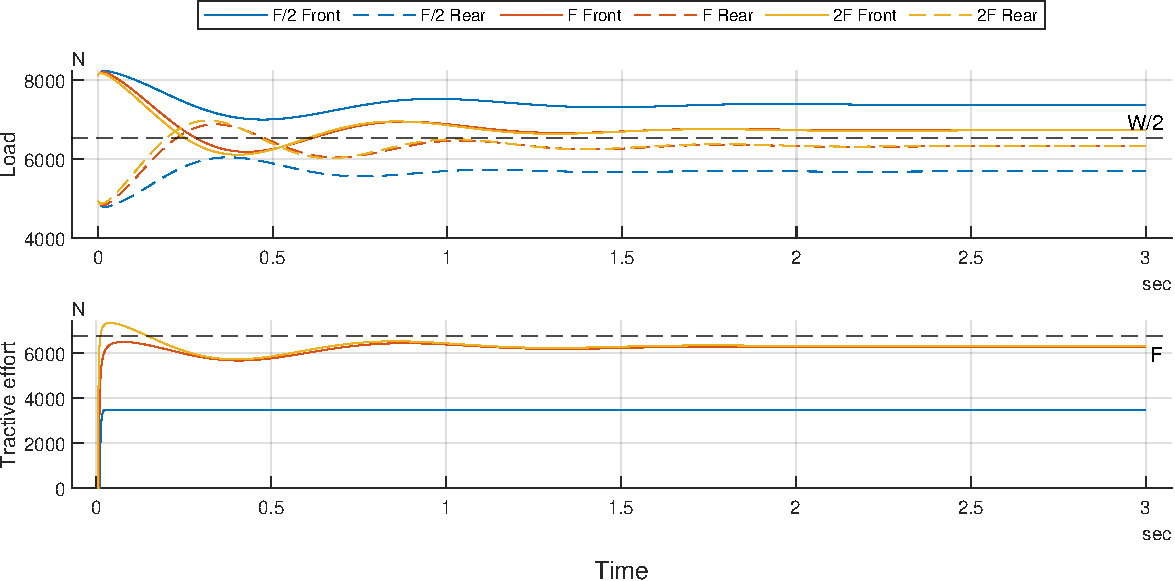
\includegraphics[width=\linewidth]{fig/fwd_traction.pdf}
	\caption{FWD traction history}
\end{figure}

The front-wheel driving results are consistent with expectation. The tractive
effort saturates at close to the calculated maximum. The equilibrium load is
biased towards the front as calculated in Eq. \ref{eq:equilibrium}, but gap
closes as the acceleration loads the rear wheels.

\begin{figure}[H]
	\centering
	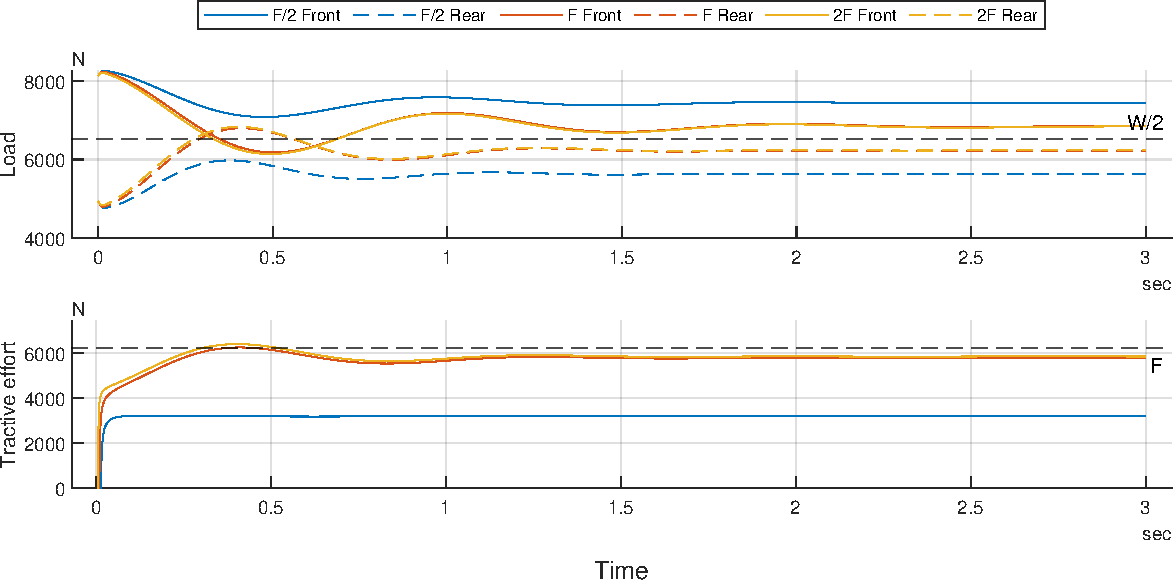
\includegraphics[width=\linewidth]{fig/rwd_traction.pdf}
	\caption{RWD traction history}
\end{figure}

Rear-wheel driving also behaves as expected, in the same ways.

\subsection{Steady-state Cornering}

The cornering stiffness implied by Eq. \ref{eq:cornering} is just \(\mu_p W\),
so the under-steer coefficient is zero. This sets the front steer angle
\cite{wongturns},

\begin{equation}
	\delta_f = \frac{L}{R} + K_\text{us} \frac{v^2}{gR} = \frac{L}{R}
\end{equation}

% The respective per-wheel loads are known from Eq. \ref{eq:equilibrium}, so the
% For this test, we use a turning radius of 

This test uses a turning radius of \SI{500}{m}, speed \SI{20}{m/s}, . The front
steering angle is \SI{0.306}{\degree} and the expected sideslip angles to
maintain this speed are \SI{4.67}{\degree}. The car is set in motion, the wheels
are deflected, and the turning is allowed to reach steady state. There is an
additional torque \(rF_x\sin(\delta_f)\) input to the rear wheels to stay close
to the intended steady state, calculated from the component of front wheel
cornering force pointed backwards due to the steering angle.

\begin{figure}[H]
	\centering
	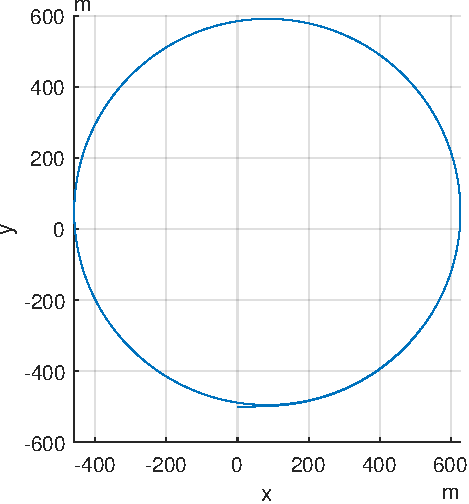
\includegraphics[height=1.5in]{fig/trajectory.pdf}
	\caption{Trajectory for verification}
\end{figure}

The trajectory matches the intended circle.

\begin{figure}[H]
	\centering
	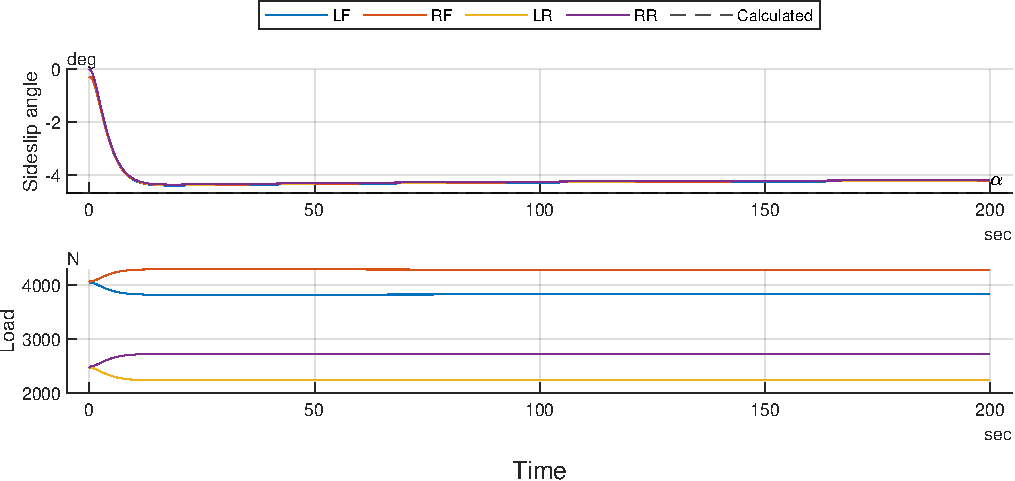
\includegraphics[width=\linewidth]{fig/circle_forces.pdf}
	\caption{Sideslip angles and load transfer}
\end{figure}

The sideslip angle remains close to expectation, but is somwhat lower because
the vehicle slowed down from steady state slightly. 

\subsection{Notes}
\begin{enumerate}
	\item The tire model is extremely stiff (in the numerical sense of having
		distant eigenvalues). A minor error between \(\omega\) and \(\vec{v}\)
		rapidly drives both quantities together, but the solver almost always
		overshoots and the result is significant chatter near either zero. This
		chatter increases if \(\epsilon\) decreases to improve accuracy. A stiff
		solver, which attempts to find the equilibrium point of that chatter, is
		required for full-vehicle simulation in any reasonable amount of time. I
		used \verb|ode15s|, which takes three orders of magnitude fewer time
		steps than \verb|ode45| with the same relative error tolerance (see
		Appendix \ref{stiffcompare}).

	\item While the traction model is `fudged' to limit the project's scope, it
		is very self-contained in terms of the slip, sideslip, and load and is
		in principle easy to replace with a more accurate model.

	\item In the same way, the vertical deflection calculation can have a
		constant or position-dependent lookup added to it to represent terrain.
\end{enumerate}


\end{multicols*}

\pagebreak
\appendix
\begin{center}
	\Large \bf Appendix
\end{center}
\section{Traction model} \label{stiffcompare}
The traction model is tested by setting a vehicle's mass in motion under a
constant load and comparing the result to a direct calculation from torque. 

\begin{figure}[H]
	\centering
	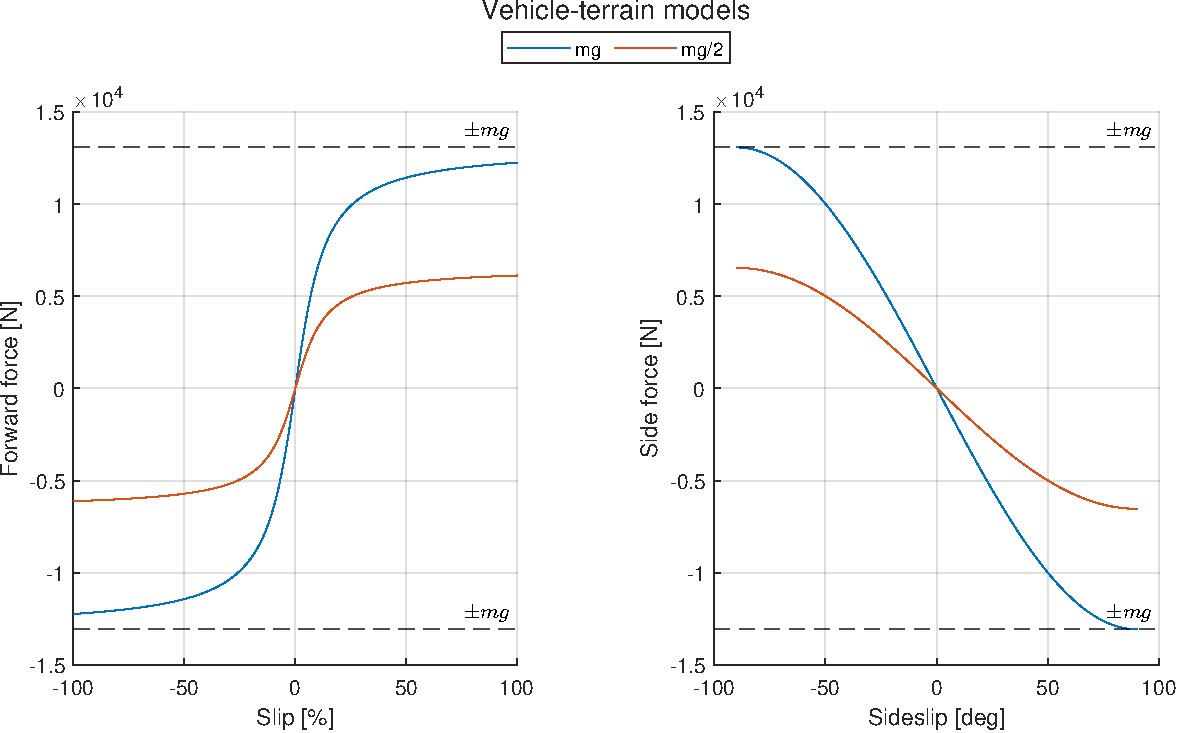
\includegraphics[height=2.5in]{fig/traction.pdf}
	\caption{Traction model}
\end{figure}

\begin{figure}[H]
	\centering
	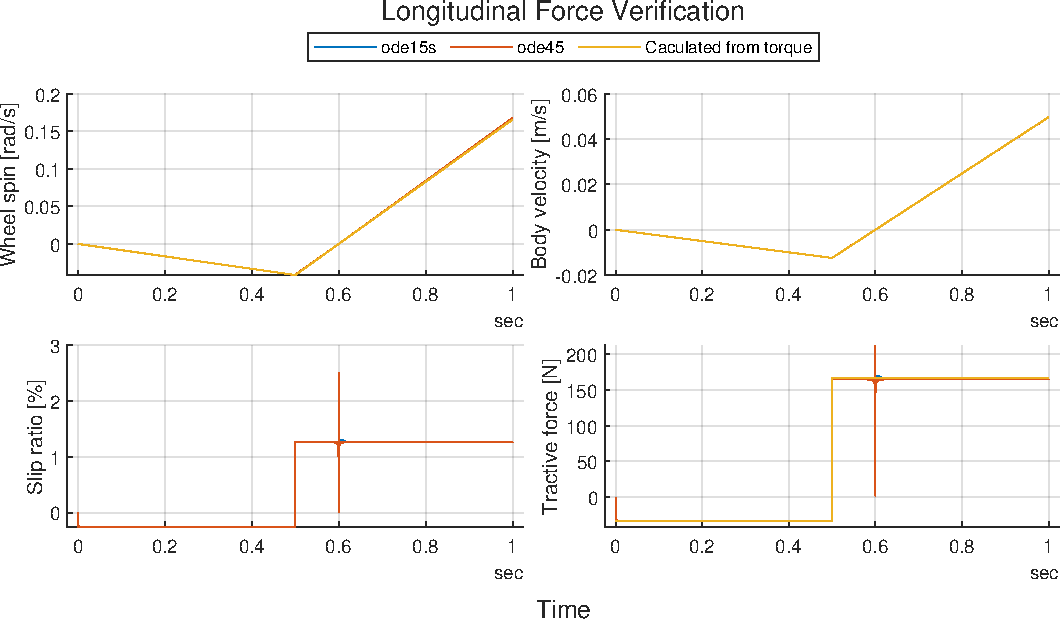
\includegraphics[height=2.5in]{fig/nominal_wheel.pdf}
	\caption{Nominal wheel operation}
\end{figure}

The calculation and computations substantially agree. However, it takes
\verb|ode45| 2 million time steps in 20 seconds of computation against
\verb|ode15s|'s 300 in 420 milliseconds for a relative error tolerance of
\(10^{-8}\). Near the zero cross, the chatter is evident.

\begin{figure}[H]
	\centering
	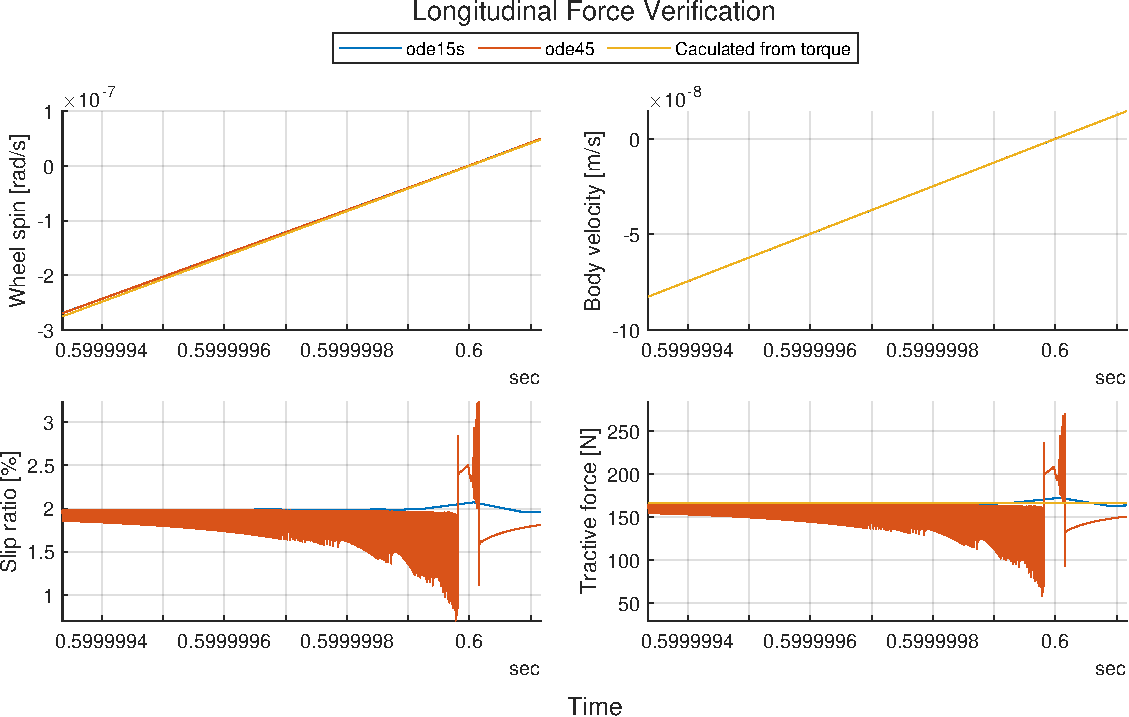
\includegraphics[height=2.5in]{fig/chatter_demo.pdf}
	\caption{Stiff system chatter}
\end{figure}

With enough torque, the traction limit is reached and the wheel spins up without
limit.
\begin{figure}[H]
	\centering
	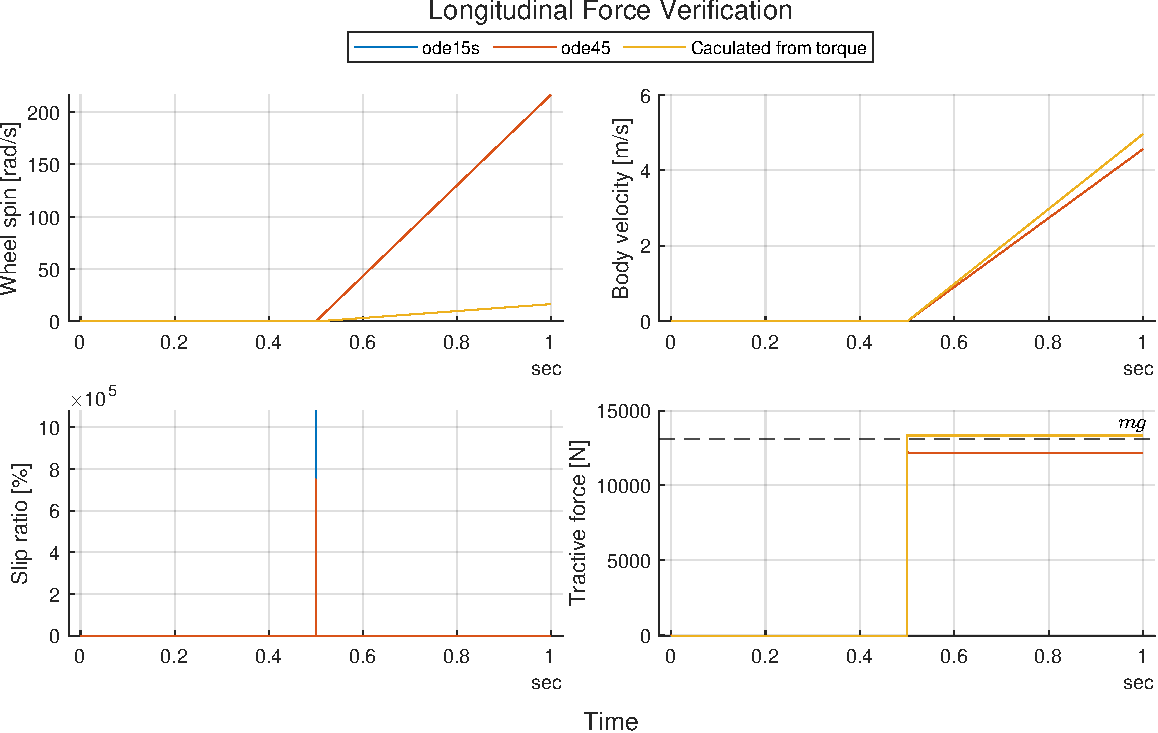
\includegraphics[height=2.5in]{fig/saturated_wheel.pdf}
	\caption{Traction-limited}
\end{figure}

\begin{landscape}
\section{Simulink Block Diagrams}

\begin{figure}[H]
	\centering
	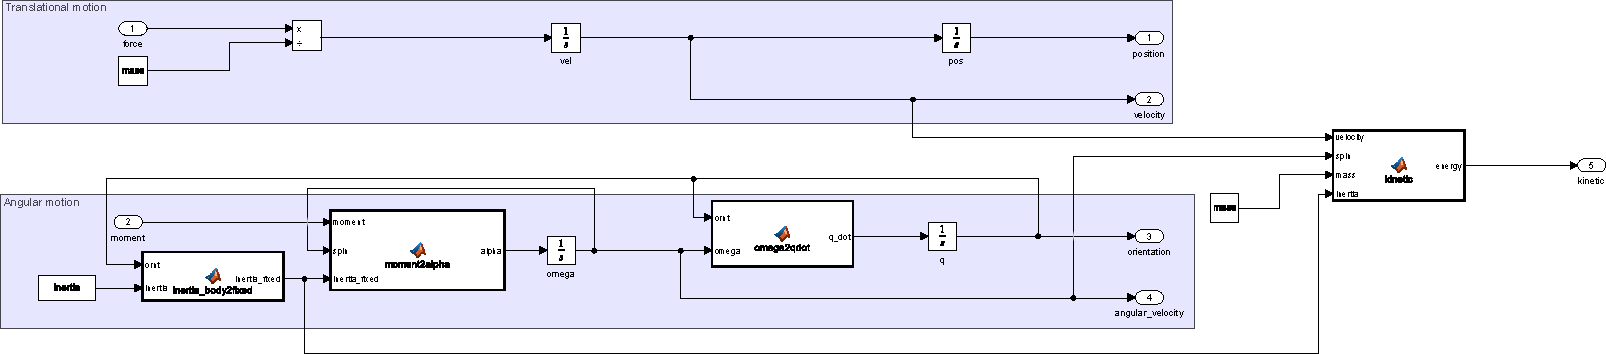
\includegraphics[width=\linewidth]{fig/rigid_body_sixdof.pdf}
	\caption{Rigid body kinetics}
\end{figure}

\begin{figure}[H]
	\centering
	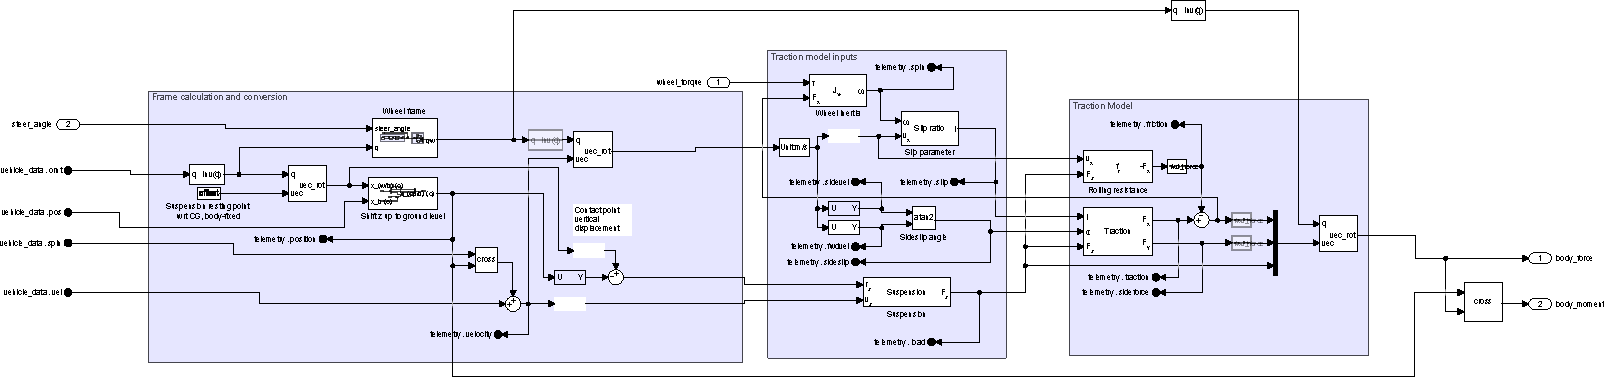
\includegraphics[width=\linewidth]{fig/quarter_car_diagram.pdf}
	\caption{Quarter-car forces}
\end{figure}

\begin{figure}[H]
	\centering
	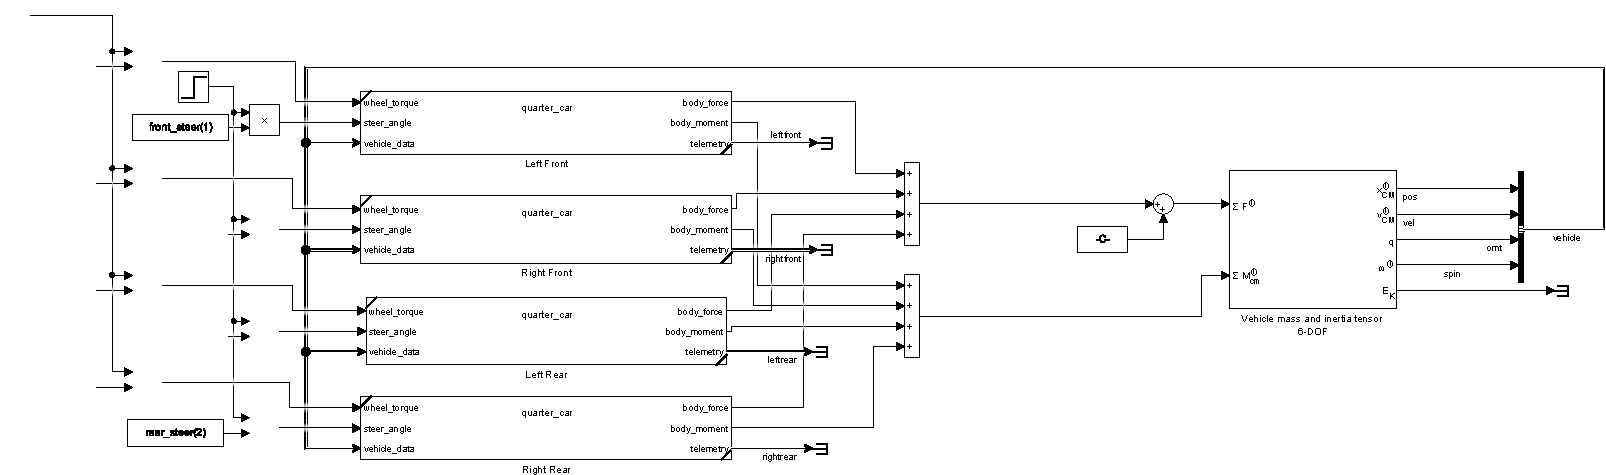
\includegraphics[width=\linewidth]{fig/vehicle_assembly.pdf}
	\caption{Assembly}
\end{figure}
	
\end{landscape}

\pagebreak
\printbibliography


\end{document}
